\documentclass[nooutcomes]{ximera}

\input{../preamble.tex}
\author{Elizabeth Miller}
\license{Creative Commons Attribution-ShareAlike 4.0 International License}
\acknowledgement{url of source material}

\title{Minimal Working Example}

\begin{document}
\begin{abstract}
  What this textbook section is about.  One or two sentences.
\end{abstract}
\maketitle


%\typeout{************************************************}
%\typeout{Motivating Questions}
%\typeout{************************************************}

\begin{motivatingQuestions}\begin{itemize}
%Often start a section. 
\item Question 1
\item Question 2
\end{itemize}\end{motivatingQuestions}


%\typeout{************************************************}
%\typeout{Introduction}
%\typeout{************************************************}



%\typeout{************************************************}
%\typeout{section}
%\typeout{************************************************}

\section{Subsection Title}
Start every file with a section.

%\typeout{************************************************}
%\typeout{Problem Types in the Text}
%\typeout{************************************************}

\section{Problem Types in the Text}

\begin{exploration}
This is a question where the answer is not proviced in the text.  The idea is that students will work on together in lecture.  It often motivates the upcoming content.
	\begin{enumerate}[label=\alph*.]
	\item Problem 1
	\item Problem 2
	\end{enumerate}
\end{exploration}


\begin{problem}
Use a Problem when students are supposed to enter an answer.  These should be straightforward things or the answer should be in a hint or explanation.  And the answer should be given in the printed text.  
$y=\answer{10x}$
	\begin{hint}
	Hint here
	\end{hint}
	\begin{explanation}
	One approach to pattern recognition is to look for a relationship in each row. Here, the $y$-value in each row is always 10 more than the $x$-value. So the pattern is described by the equation $y=10x$
	\end{explanation}
\end{problem}


\begin{example}
A standard example with solution in the text.
	\begin{explanation}
	Every example should have an explanation.
	\end{explanation}
\end{example}


%\typeout{************************************************}
%\typeout{Other Environments in Text}
%\typeout{************************************************}

\section{Other Environmentsin the Text}

\begin{remark}
Something you want to call attention to in the text.
\end{remark}


\begin{definition}
Define a word or words.  Be sure to use the dfn command around your \dfn{vocab words}.
\end{definition}


\begin{callout}
Something that you want to standout that is not a remark.  Basically just puts it in a blue box.
\end{callout}

\begin{summary}
  %Often ends a section
  \begin{itemize}
\item First point
\item Second point
  \end{itemize}
\end{summary}


%\typeout{************************************************}
%\typeout{Tables and Graphs}
%\typeout{************************************************}

\section{Tables and Graphs}

How to make a table:


$$
\begin{array}{cc}
t&V\\
\hline
0&0.0\\
1&0.5\\
2&1.0\\
3&1.5\\
4&2.0\\
5&2.5
\end{array}
$$


Side-by-side tables (or images or whatever):


$$
\begin{array}{cccccc}
%$
{\begin{array}{cc}
t&r(t)\\
\hline
0&12\\
3&10\\
6&8\\
9&6
\end{array}}&&&&&
%$
%\end{center}
%\begin{center}
%$
{\begin{array}{cc}
t&s(t)\\
\hline
0&12\\
3&9\\
6&6.75\\
9&5.0625
\end{array}}\\
\end{array}
$$


How to make an image:
\begin{image}
\includegraphics{ColumbusChicago.png}
\end{image}


Draw graphs in tikzi when possible.  Here are two.

\begin{image}
\begin{tikzpicture}
    \begin{axis}
        \addplot[samples=200,domain=0.01:8]{ln(x)};
    \end{axis}
\end{tikzpicture}
\end{image}

\begin{image}
\begin{tikzpicture}
    \begin{axis}[xlabel={},ylabel={},width=0.75\linewidth,
                xmin=-5,xmax=5,
                ymin=-5,ymax=5,
                xtick={-4,4},
                ytick={-4,4},
                clip=false]
        \addplot[soliddot] coordinates {(0,0)} node[pin=240:{Carl's house}] {};
        \addplot[soliddot] coordinates {(2, 3)} node[pin=-30:{restaurant}] {};
        \addplot[soliddot] coordinates {(-3, 2)} node[pin=100:{pet shop}] {};
        \addplot[soliddot] coordinates {(-2, -4)} node[pin=150:{gas station}] {};
        \addplot[soliddot] coordinates {(3, -3)} node[pin=120:{bar}] {};
        \addplot[mark=none] coordinates {(5, 0)} node[above left] {east};
        \addplot[mark=none] coordinates {(-5, 0)} node[above right] {west};
        \addplot[mark=none] coordinates {(0, 5)} node[below right] {north};
        \addplot[mark=none] coordinates {(0, -5)} node[above right] {south};
    \end{axis}
\end{tikzpicture}
\end{image}


You can also add Desmos interactives.  Create them in a Desmos account (I think we have an OSU one.  We should look into that!).  Save them.  Then pull the graph number out of the url.
\begin{center}  
\desmos{lxllnpdi6w}{800}{600}  
\end{center}

Here is a tikz unit circle which can be editted easily.  Creative Commons, Citation: https://texample.net/tikz/examples/unit-circle/

\scalebox{0.75}{
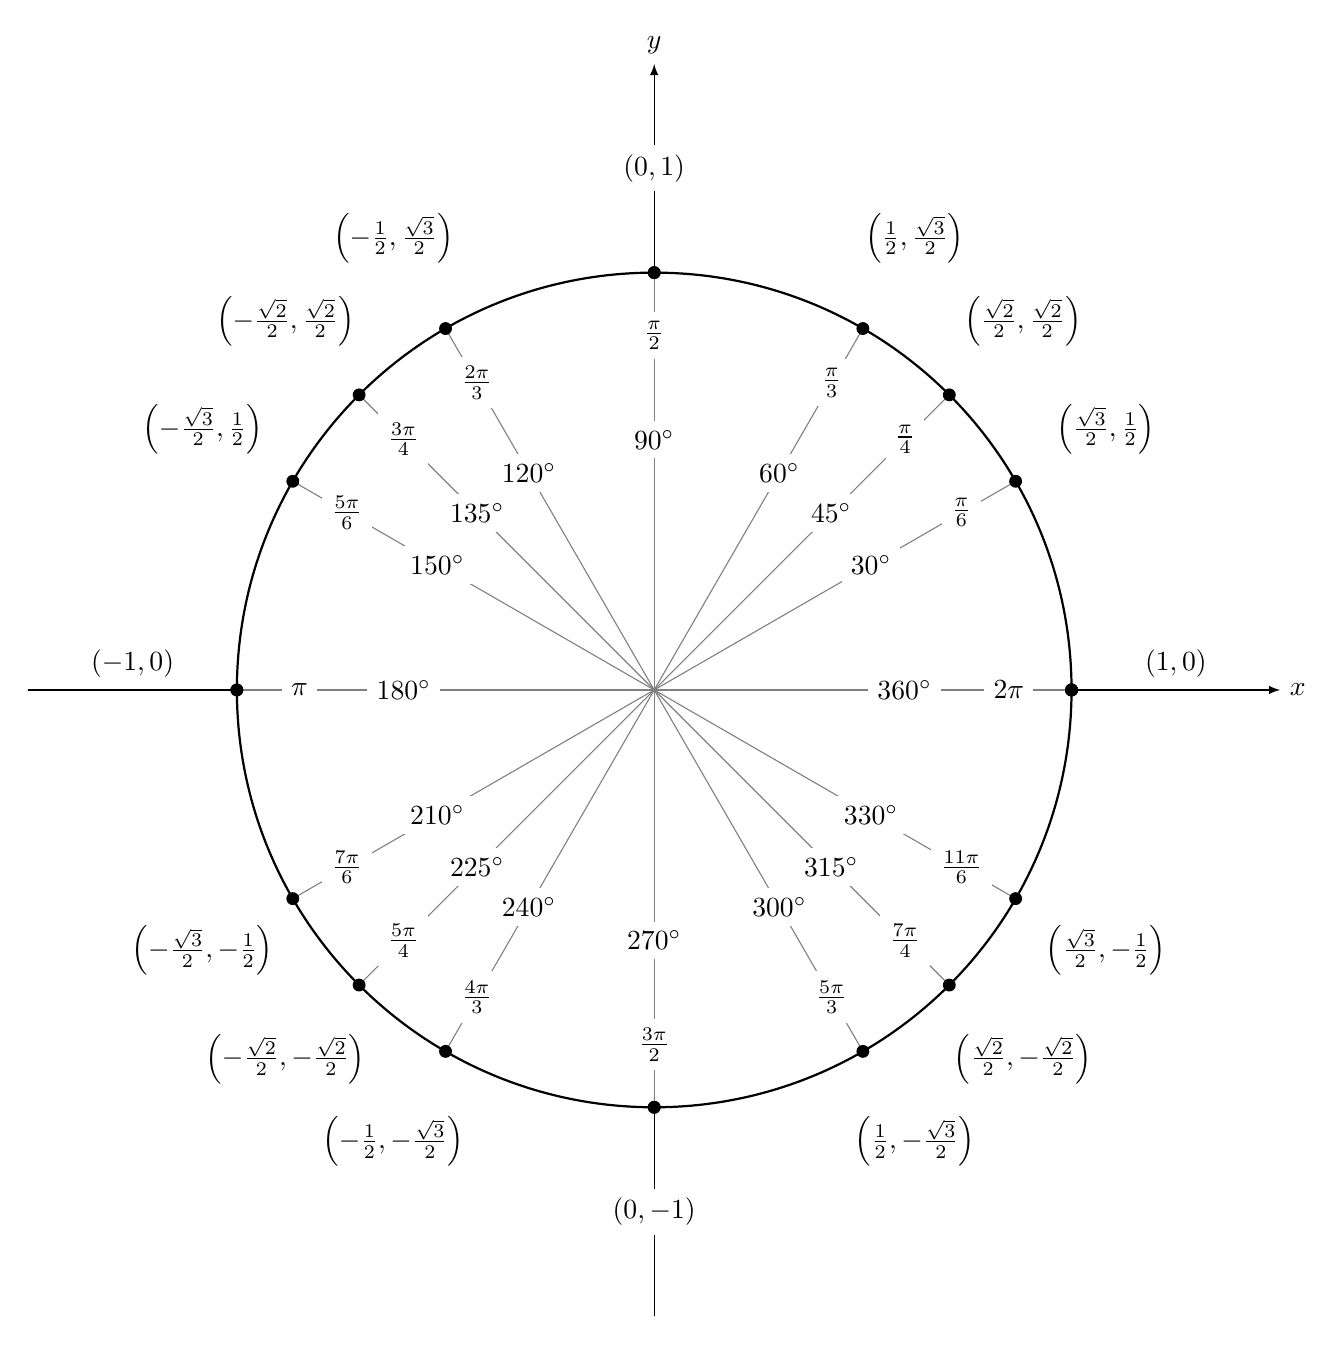
\begin{tikzpicture}[scale=5.3,cap=round,>=latex]
        % draw the coordinates
        \draw[->] (-1.5cm,0cm) -- (1.5cm,0cm) node[right,fill=white] {$x$};
        \draw[->] (0cm,-1.5cm) -- (0cm,1.5cm) node[above,fill=white] {$y$};

        % draw the unit circle
        \draw[thick] (0cm,0cm) circle(1cm);

        \foreach \x in {0,30,...,360} {
                % lines from center to point
                \draw[gray] (0cm,0cm) -- (\x:1cm);
                % dots at each point
                \filldraw[black] (\x:1cm) circle(0.4pt);
                % draw each angle in degrees
                \draw (\x:0.6cm) node[fill=white] {$\x^\circ$};
        }

        \foreach \x in {0,45,...,360} {
                % lines from center to point
                \draw[gray] (0cm,0cm) -- (\x:1cm);
                % dots at each point
                \filldraw[black] (\x:1cm) circle(0.4pt);
                % draw each angle in degrees
                \draw (\x:0.6cm) node[fill=white] {$\x^\circ$};
        }

        % draw each angle in radians
        \foreach \x/\xtext in {
            30/\frac{\pi}{6},
            45/\frac{\pi}{4},
            60/\frac{\pi}{3},
            90/\frac{\pi}{2},
            120/\frac{2\pi}{3},
            135/\frac{3\pi}{4},
            150/\frac{5\pi}{6},
            180/\pi,
            210/\frac{7\pi}{6},
            225/\frac{5\pi}{4},
            240/\frac{4\pi}{3},
            270/\frac{3\pi}{2},
            300/\frac{5\pi}{3},
            315/\frac{7\pi}{4},
            330/\frac{11\pi}{6},
            360/2\pi}
                \draw (\x:0.85cm) node[fill=white] {$\xtext$};

        \foreach \x/\xtext/\y in {
            % the coordinates for the first quadrant
            30/\frac{\sqrt{3}}{2}/\frac{1}{2},
            45/\frac{\sqrt{2}}{2}/\frac{\sqrt{2}}{2},
            60/\frac{1}{2}/\frac{\sqrt{3}}{2},
            % the coordinates for the second quadrant
            150/-\frac{\sqrt{3}}{2}/\frac{1}{2},
            135/-\frac{\sqrt{2}}{2}/\frac{\sqrt{2}}{2},
            120/-\frac{1}{2}/\frac{\sqrt{3}}{2},
            % the coordinates for the third quadrant
            210/-\frac{\sqrt{3}}{2}/-\frac{1}{2},
            225/-\frac{\sqrt{2}}{2}/-\frac{\sqrt{2}}{2},
            240/-\frac{1}{2}/-\frac{\sqrt{3}}{2},
            % the coordinates for the fourth quadrant
            330/\frac{\sqrt{3}}{2}/-\frac{1}{2},
            315/\frac{\sqrt{2}}{2}/-\frac{\sqrt{2}}{2},
            300/\frac{1}{2}/-\frac{\sqrt{3}}{2}}
                \draw (\x:1.25cm) node[fill=white] {$\left(\xtext,\y\right)$};

        % draw the horizontal and vertical coordinates
        % the placement is better this way
        \draw (-1.25cm,0cm) node[above=1pt] {$(-1,0)$}
              (1.25cm,0cm)  node[above=1pt] {$(1,0)$}
              (0cm,-1.25cm) node[fill=white] {$(0,-1)$}
              (0cm,1.25cm)  node[fill=white] {$(0,1)$};
    \end{tikzpicture}
}


%\typeout{************************************************}
%\typeout{Online Features}
%\typeout{************************************************}

\section{Online Features}

To add a url, use the link command.
For more about formatting in Ximera see \link[this url]{https://ximera.osu.edu/intro/gettingStarted/graphicsAndVideos/graphicsAndVideos}.


You can also embed \link[YouTube]{https://www.youtube.com/} videos.
\begin{center}
\youtube{0aQpLSu2fMs}
\end{center}





\newpage

%\typeout{************************************************}
%\typeout{Overviews}
%\typeout{************************************************}

\section{Overviews}

Each Unit has an overview with the organization and learning objectives

\begin{overview}\begin{itemize}
\item Generally a folder %(author if relevant)
	\begin{enumerate}
	\item some stuff covered in these sections
		\textit{a subtopic} 
		\textit{another subtopic} 
	\item More stuff	
	\end{enumerate}	
\item Another Folder 
	\begin{enumerate}	
	\item Stuff 
	\end{enumerate} 
\end{itemize}\end{overview}


\begin{objectives}
\item Learning Objectives Category (Course level learning objective)
	\begin{itemize}
	\item more specific goal
	\item another one 
	\end{itemize}
\item Another Category
	\begin{itemize}
	\item Linear 
	\item Parabolas 
	\item Polynomials 
	\end{itemize}
\end{objectives}




\newpage

%\typeout{************************************************}
%\typeout{Homeworks}
%\typeout{************************************************}

\section{Homework}
Each homework problem should be it's own file.  Then the homework is put together using an exerciselist file.  See a Unit 1 folder for an example.  Be sure to keep all the same conventions, just changing the actual problem.  

Some Ximera problem types are available \link[in the footnote]{https://ximera.osu.edu/intro/gettingStarted/questionAndAnswerTypes/questionAndAnswerTypes}.  We can add more here as we come across them.


%\typeout{************************************************}
%\typeout{Labeling and Referencing}
%\typeout{************************************************}
\section{Labeling and Referencing}

Depending upon how a source file is compiled, the numbering of examples may be changed. When compiling a single source file, this could be a small value,
but when included and compiled as a larger file or as other examples are included, that number could change. Using Labels and References will allow us to 
refer to the examples by number in the text, but will adjust the numbering of those references to match the numbering of the example at compile-time.


Adjusting the numbering for exercises is handled through labels ( using the $\backslash$\emph{label} command ) and references (using the $\backslash$\emph{ref} command ). 
The $\backslash$label command adds a virtual label (which you have to give a name for), which identifies the counter associated with the object you're labelling. It doesn't typeset anything, just identifies the value of that particular counter with the name of the label. 
The $\backslash$ref command prints out the value of that label (you have to reference the name of the label you have previously created).

For example, here is a sample example:
\begin{example}\label{example:SampleExample}
	A Sample example is here
\end{example}

In the code, immediately after $\backslash$begin\{example\} (but before the text of the example), you'll see 
$\backslash$label\{example:SampleExample\}. This creates the label for the 
example counter that we've named \emph{example:SampleExample}. (It could have been named something as simple as ``\emph{Ex}'' or ``\emph{a}''. 
The name ``\emph{example:SampleExample}'' was picked for readability.) 
The counter value is set at that $\backslash$\emph{begin\{example\}} statement, so your $\backslash$\emph{label} should be immediately after it,
before any other text.


When we want to reference this example later, we have to use $\backslash$ref\{example:SampleExample\}, which here has value \ref{example:SampleExample},

This means the code ``Example $\backslash$ref\{example:SampleExample\}'' is typeset as ``Example \ref{example:SampleExample}''. 
The numbering will be updated according to how the Example is numbered when compiled. 

\begin{callout}
	In order for this referencing to work, you have to compile the source file TWICE!
\end{callout}

The first time through, the compiler will assign values to the counters and store the values of the labels in the aux files it generates. The second time
through, the compiler will actually add the values of those references to the typeset document. (This is a standard issue for virtually all compilers with 
preprocessing options. Most run twice automatically, but LaTeX/pdfLaTeX  defaults to only running once.) If you see the references showing up as 
question marks instead of as numbers, try compiling another time or two.

In \LaTeX,  captions/labels/references are for figures, not for images or tikzpictures. To add a caption/label/reference for a graph, it has to be in an outer
 \emph{figure} environment, so put the whole thing inside an $\backslash$\emph{begin\{figure\}} ... $\backslash$\emph{end\{figure\}} block. 
 LaTeX  places figures wherever it decides is best, not based on where it appears in the source file. You can demand it to go where it appears in the source 
 by using the option \emph{!h}. This makes the opening tag look like: $\backslash$\emph{begin\{figure\}[!h]}. 
 (The exclamation point is an override to the default \emph{figure} setup, and the h says you want the figure \emph{here}.)

\begin{figure}[!h]
	\begin{image}
		\begin{tikzpicture}
		    \begin{axis}
        		\addplot[samples=200,domain=0.01:8]{ln(x)};
    			\end{axis}
		\end{tikzpicture}
	\end{image}
	\caption{Here is an example graph}
	\label{fig:pic}
\end{figure}

The last three lines should be the $\backslash$\emph{caption}\{ ... \}, followed by $\backslash$\emph{label}\{...\}, then the $\backslash$\emph{end\{figure\}}. 
The order here is important. The caption statement has to come before the label.

Referencing these figures is exactly the same as with examples: Here was Figure \ref{fig:pic}

\end{document}
